\chapter{ΑΝΑΣΚΟΠΗΣΗ ΤΩΝ ΑΡΘΡΩΝ}

\section{ΠΡΟΣΕΓΓΙΣΕΙΣ ΜΕ ΒΑΣΗ ΤΗΝ XML}
    Το άρθρο "\textit{XML-based approaches for the integration of heterogeneous bio-molecular data}" των Mesiti, Jimenez-Ruiz κ.α. πραγματεύεται κάποιες προσεγγίσεις για την αναπαράσταση, ενσωμάτωση και διαχείριση βιολογικών δεδομένων με τη χρήση γλωσσών που βασίζονται στην XML.
    Επιπλέον, παρουσιάζεται μια νέα προσέγγιση για τη διαχείριση ετερογενών βιολογικών δεδομένων μέσω της XML. \cite{XMLbasedApproaches}
    
    \subsection{Χρησιμότητα XML}
        Η XML έχει αναδειχθεί ως την πιο αποτελεσματική πρόταση για την αναπαράσταση δομημένων πληροφοριών, μιας και επιτρέπει την εύκολη επέκταση και τροποποίηση, κάτι βολικό μιας και καθημερινά δημιουργούνται και αναπτύσσονται νέα βιολογικά δεδομένα.
        Υποστηρίζεται από γλώσσες ερωτημάτων (query languages) όπως η XPath και XQuery, δίνοντας τη δυνατότητα για άμεση εξόρυξη των πληροφοριών.

        Χρησιμοποιεί μια ιεραρχική δόμηση της πληροφορίας με στοιχεία (XML Elements), χαρακτηριστικά (XML attributes) και κείμενο (XML text content).
        Κάθε στοιχείο μπορεί να αναπαριστά κάποια συγκεκριμένη βιολογική οντότητα (πχ DNA, RNA, πρωτεΐνη) και μπορεί να περιλαμβάνει εμφωλευμένα στοιχεία για συσχετιζόμενα χαρακτηριστικα.
        Αυτή η ιεραρχική δόμηση επιτρέπει την αναπαράσταση με σαφήνεια πολύπλοκων βιολογικών σχέσεων.


    \subsection{Βιολογικοί τύποι δεδομένων}
        Το άρθρο παρουσιάζει κάποιους τύπους βιολογικών δεδομένων. Για παράδειγμα:
    \begin{itemize}[label={\tiny \blacksquare}]
        \vspace{-10pt}
        \item \textbf{Δεδομένα πρωτοταγών πρωτεϊνών}: περιλαμβάνουν δεδομένα νουκλεοτιδικών αλληλουχιών, φιλοξενούνται σε βάσεις δεδομένων όπως GenBank και EMBL.
        \item \textbf{Δεδομένα πρωτεϊνών}: βάσεις δεδομένων όπως SWISSPROT και TREMBL περιέχουν πληροφορίες για πρωτεϊνικές αλληλουχίες, αναπαρίστανται εύκολα σε XML.
        \item \textbf{Motif (μοτίβα) και πρωτεϊνικές περιοχές}: προσδιορίζονται μέσω μεθόδων αναγνώρισης προτύπων που εφαρμόζονται σε δεδομένα πρωτοταγών πρωτεϊνών, αναπαρίστανται με μια περιγραφή του μοτίβου, βιβλιογραφικές πληροφορίες κ.α.
    \end{itemize}


    \subsection{Αναπαράσταση βιολογικών δεδομένων με τη χρήση XML}
        Έχουν χρησιμοποιηθεί αρκετές γλώσσες βασισμένες στην XML, ειδικά για την αναπαράσταση διαφορετικών τύπων βιολογικών δεδομένων. Για παράδειγμα:

        \subsubsection{Bioinformatic Sequence Markup Language (BSML)}
            Γλώσσα σχεδιασμένη για να περιγράφει αλληλουχίες όπως DNA, RNA και πρωτεϊνικές αλληλουχίες.
            Ένα BSML αρχείο περιλαμβάνει πληροφορίες για το πώς τα γονιδιώματα κωδικοποιούνται, ανακτώνονται και εμφανίζονται.

        \subsubsection{Protein Markup Language - ProXML}
            Χρησιμοποιείται για την αναπαράσταση πρωτεϊνικών αλληλουχιών.
            Περιλαμβάνει ένα identity section που περιέχει την περιγραφή των πρωτεϊνών και ένα data section που περιέχει ιδιότητες από αυτές τις πρωτεΐνες.

        \subsubsection{ΠΡΟΕΚΤΑΣΗ: RNA Markup Language - RNAML}
            Γλώσσα που σχεδιάστηκε με σκοπό να διευκολύνει την ανταλλαγή RNA πληροφοριών μεταξύ διαφορετικών λογισμικών βιοπληροφορικής. \cite{RNAML}
            Μέχρι πρότινος, κάθε εργαστήριο ανέπτυσσε το δικό του λογισμικό με τους δικούς του τύπους αρχείων για την ανάγνωση και την εγγραφή της βιοπληροφορίας.
            Επομένως, κατέστη αναγκαία η δημιουργία μιας τυποποίησης της RNA πληροφορίας, με σκοπό την αύξηση της αποτελεσματικότητας στην κοινότητα των βιολόγων.

            Οι προηγούμενες προσπάθειες για τυποποίηση της βιολογικής πληροφορίας περιλαμβάνουν τη γλώσσα σήμανσης BIOpolymer Markup Language (BIOML)  η οποία αναπτύχθηκε το 1999 από την ProteoMaterics.
            Περιλαμβάνει ένα framework για τον καθορισμό μοριακών οντοτήτων, και ενώ περιλάμβανε κάποιες πληροφορίες για το RNA, εστιάζονταν περισσότερο στη γονιδιακή του πλευρά
                (θέσεις έναρξης και παύσης της μεταγραφής, γενετικές τροποποιήσεις κτλ), και δεν κάλυπτε επαρκώς πληροφορίες για τη δομή του RNA, κάτι ερευνητικά κρίσιμο.
            Γενικότερα οι προηγούμενες προσπάθειες δεν κάλυπταν τις απαιτήσεις που έθετε η επιστημονική κοινότητα που μελετούσε το RNA, οδηγώντας στην ανάπτυξη της RNAML.

            Η RNAML βασίζεται πάνω στο XML.
            Υπάρχει η δυνατότητα δημιουργίας ενός Document Type Definition (DTD) το οποίο καθορίζει τη δομή του εγγράφου, τα ονόματα και τον τύπο των στοιχείων και τη ιεραρχική δομή τους,
                κάτι που διασφαλίζει τη συνέπεια και τη συμμόρφωση στο πώς αναπαρίσταται το RNA.
            Επίσης, μπορεί να αναπαριστά την αλληλεπίδραση πολλαπλών μορίων RNA, την απόσταση τους, τη σύζευξη των βάσεών τους, και οποιαδήποτε άλλη σχέση έχουν μεταξύ τους.
            Τέλος, πέρα από δυνατότητες για σχολιασμό (annotation) και documentation σε κάθε στοιχείο, είναι δυνατή η ομαδοποίηση των εμφανίσεων του ίδιου λειτουργικού RNA σε διαφορετικούς οργανισμούς,
                κάνοντας εφικτή την αναπαράσταση ευθυγραμμίσεων και κοινών δομικών συστατικών.

        \subsubsection{ΠΡΟΕΚΤΑΣΗ: System Biology Markup Language (SBML)}
            Δημιουργήθηκε στα πλαίσια του ERATO Kitano Systems Biology Project για να διευκολύνει την ανταλλαγή μοντέλων μεταξύ διαφορετικών εργαλείων προσομοίωσης και ανάλυσης. \cite{SBML}

            Ένα SBML μοντέλο περιλαμβάνεται από το Διαμέρισμα (Compartment), έναν καθορισμένο χώρο όπου συμβαίνουν οι αντιδράσεις όπως ένα κύτταρο ή ένα οργανίδιο,
                ένα Eίδος (Species), οι χημικές οντότητες που συμμετέχουν στις αντιδράσεις όπως τα ιόντα ή τα μόρια, η Αντίδραση (Reaction), η διαδικασία σχηματισμού μεταξύ των ειδών,
                η Παράμετρος (Parameter), η οποία αναπαριστά ποσότητες με συμβολικά ονόματα τοπικά η καθολικά, οι Ορισμοί Μονάδων (Unit Definitions), για τον προσδιορισμό των μονάδων που χρησιμοποιούνται στο μοντέλο,
                και τέλος οι Κανόνες (Rules), μαθηματικές εκφράσεις που ορίζουν τις τιμές των παραμέτρων ή θέτουν περιορισμούς στο μοντέλο.

            \begin{figure}[ht] \noindent\centering
                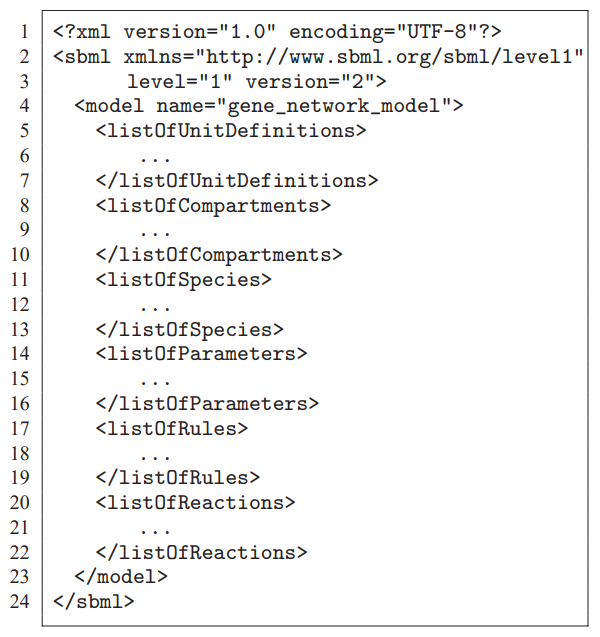
\includegraphics[scale=0.7]{img/SBML skeleton}
                \caption{Σκελετός από τον ορισμό ενός μοντέλου SBML \cite{SBML}}
            \end{figure}

        \subsubsection{ΠΡΟΕΚΤΑΣΗ: Cell Markup Language (CellML)}
            Το CellML προσφέρει μια σαφή μέθοδο ορισμού μοντέλων κυτταρικής λειτουργίας, σε ένα πιο γενικό πλαίσιο σε σχέση με τα προηγούμενα. \cite{CellML}
            Το βάθος στο οποίο μπορεί το CellML να αναπαραστήσει τις έννοιες επικαλύπτει γλώσσες όπως η SBML, με τη διαφορά ότι η SBML βασίζεται περισσότερο
                στην περιγραφή βιοχημικών αντιδράσεων, χάνοντας πληροφορία για τη δομή των μοντέλων.

            Η CellML από την αρχή σχεδιάστηκε για να υποστηρίξει μοντέλα μεγάλης κλίμακας, επιτρέπεται (λόγω της XML βάσης της) η ανεξάρτητη κατασκευή μοντέλων και τμημάτων
                και η ενσωμάτωσή τους σε ένα μεγαλύτερο μοντέλο, και παρέχει τρόπους για την απόκρυψη low-level πληροφοριών ώστε να μη συγχέονται με το υψηλότερο επίπεδο αναπαράστασης του μοντέλου.

            \begin{figure}[ht] \noindent\centering
                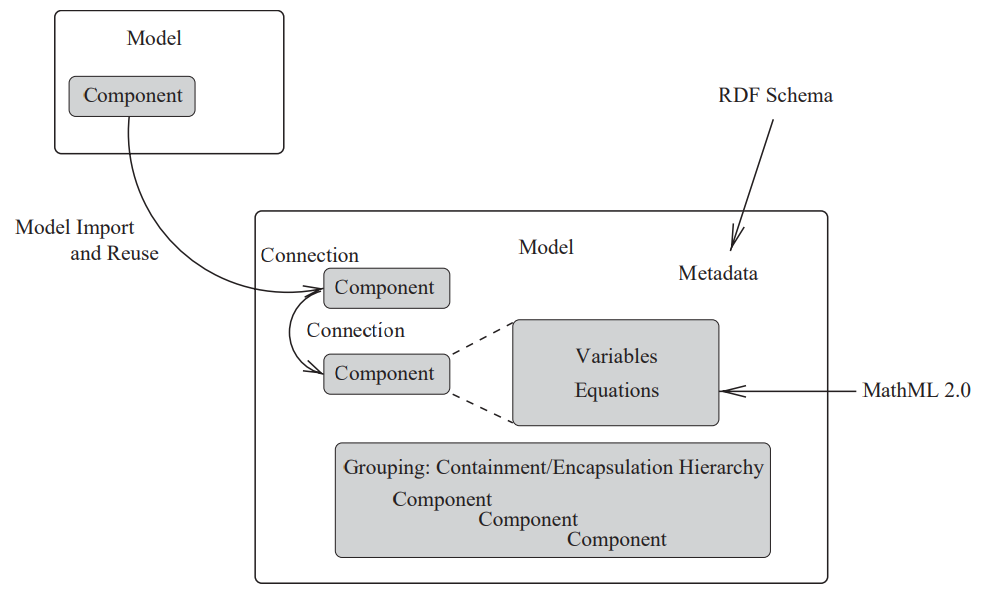
\includegraphics[scale=0.7]{img/CellML structure}
                \caption{Διάγραμμα με το σκελετό ενός CellML μοντέλου \cite{CellML}}
            \end{figure}


    \subsection{Διαχείριση ετερογενών βιολογικών δεδομένων}
        Οι βιολόγοι συνήθως χρησιμοποιούν διαφορετικές βάσεις δεδομένων, η κάθε μία με το δικό της σχεδιασμό της πληροφορίας, που καθιστά χρονοβόρα την ανάκτηση πληροφορίας.
        Επομένως, είναι αυξημένη η ανάγκη για πρόσβαση σε μια ομογενοποιημένη βάση δεδομένων, κάτι που δεν είναι πάντα εύκολο να επιτευχθεί λόγω της ετερογένειας της πληροφορίας.

        Λύση σε αυτό είναι η γλώσσα XML, που προφέρει έναν τρόπο για τη συντακτική ενσωμάτωση των δεδομένων, αν και στερείται των μεθόδων με τους οποίους μπορεί να επιτευχθεί αυτή η ενσωμάτωση.
        Τέτοιες μέθοδοι ονομάζονται αρχιτεκτονικές ενσωμάτωσης (integration architectures) και χωρίζονται στις Data warehouse, Mediator-based, Service-oriented και Peer-based αρχιτεκτονικές.

        Το δεύτερο μέρος του άρθρου αναλύει τη χρήση αυτών των αρχιτεκτονικών σε συνδυασμό με την XML για την ενσωμάτωση των δεδομένων.

        \subsubsection{ΠΡΟΕΚΤΑΣΗ: Data warehouse συστήματα}
        Η Data warehouse αρχιτεκτονική ενσωματώνει δεδομένα από διαφορετικές βάσεις δεδομένων σε μια, καταφέρνοντας μια υψηλότερου βαθμού ομογενοποίηση και χωρίς να χρειάζονται συχνές ανανεώσεις.
        Παραδείγματα τέτοιων συστημάτων είναι τα εξής:

            \paragraph{DWARF}
                Πρόκειται για ένα data warehouse σύστημα που σχεδιάστηκε για την ανάλυση μεγάλων πρωτεϊνικών οικογενειών.
                Ενσωματώνει δεδομένα που αφορούν την αλληλουχία, τη δομή και τον χαρακτηρισμό πρωτεϊνών, συνδυάζοντας δεδομένα από διαφορετικές δημόσιες βάσεις δεδομένων όπως GenBank, ExPDB, κ.α.

                Το σχεσιακό του μοντέλο δεδομένων αναπτύχθηκε στο Firebird, ένα ανοιχτού κώδικα σύστημα διαχείρισης σχεσιακών βάσεων SQL, και είναι οργανωμένο σε τρία μεγάλα τμήματα που αντιπροσωπεύουν διαφορετικές οντότητες:
                    την πρωτεΐνη (περιγράφει τη βιοχημική λειτουργία, τον οργανισμό προέλευσης και την ταξινόμηση των πρωτεϊνών), την αλληλουχία των πρωτεϊνών (σχολιασμός συγκεκριμένων θέσεων,
                        λεπτομέρειες για μεταλλάξεις) και δομή πρωτεΐνης (δεδομένα που σχετίζονται με τις δευτερογενείς και τριτογενείς δομές της πρωτεΐνης). \cite{DWARF}

            \paragraph{BioWarehouse}
                Πρόκειται για ένα toolkit ανοιχτού κώδικα που έχει σχεδιαστεί για τη διευκόλυνση της διασύνδεσης διαφορετικών βάσεων δεδομένων βιοπληροφορικής.
                Χρησιμοποιεί τη MySQL και την Oracle ως relational database managers, και επιτρέπει την ομαλή σύνδεση διαφορετικών βάσεων δεδομένων με σκοπό να γίνονται αποτελεσματικά queries και την εξόρυξη δεδομένων. \cite{BioWarehouse}

                Περιλαμβάνονται εργαλεία σε C και σε Java που κάνουν συντακτική ανάλυση (parsing) και κανονικοποιούν τα δεδομένα για να μειώσουν την ετερογένεια, ενώ έχει σχεδιαστεί ώστε να επιτρέπεται η κλιμάκωση για πολλά terabytes δεδομένων.
                Όλα αυτά κάνουν το BioWarehouse ένα χρήσιμο εργαλείο με πολλές πρακτικές εφαρμογές, όπως για παράδειγμα για τον προσδιορισμό κενών σε αλληλουχίες.

            \paragraph{Atlas}
                Data warehouse σύστημα που αποθηκεύει και ενοποιεί διαφορετικούς τύπους βιολογικών δεδομένων.
                Χρησιμοποιεί την SQL η οποία καλεί (μέσω API) εφαρμογές σε C++, Java και Perl γλώσσες, οι οποίες διαβάζουν πληροφορίες από άλλες βάσεις δεδομένων (GenBank, RefSeq, UniProt κ.α.) στη βάση δεδομένων του Atlas.
                Επίσης, περιλαμβάνει κάποια εργαλεία που χρησιμοποιούνται για την εξόρυξη δεδομένων. \cite{Atlas}

            \paragraph{Biozone}
                Ενοποιημένη πηγή για DNA αλληλουχίες, πρωτεΐνες κ.α., που ενσωματώνει μοντέλα γράφων και ιεραρχικές κλάσεις για την αναπαράσταση και την κατηγοριοποίηση βιολογικών οντοτήτων.

            \paragraph{cPath}
                Λογισμικό βάσης δεδομένων ανοιχτού κώδικα για τη συλλογή, αποθήκευση και αναζήτηση δεδομένων βιολογικών μονοπατιών.
                Τα δεδομένα μπορούν και προβάλλονται σε browser ή να εξαχθούν μέσω API που βασίζεται σε XML, κάτι που επιτρέπει τη χρήση του σε third-party εφαρμογές φτιαγμένες για την οπτικοποίηση και ανάλυση μονοπατιών.

            \begin{figure}[ht] \noindent\centering
                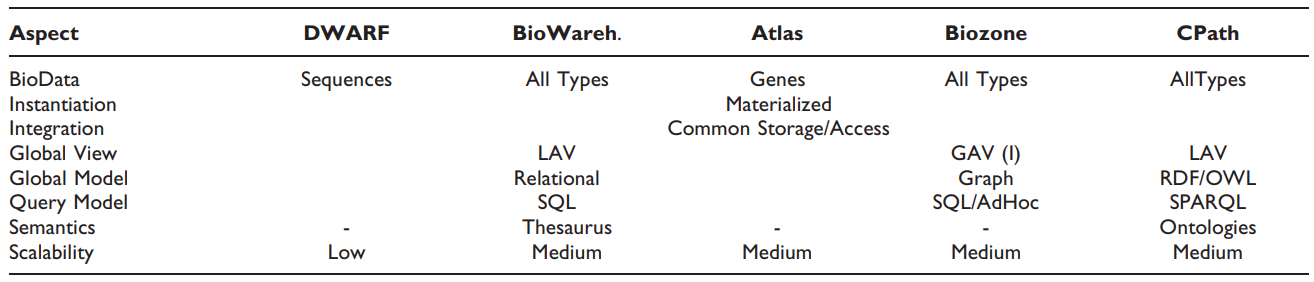
\includegraphics[scale=0.7]{img/Data warehouse table}
                \caption{Σύγκριση των Data Warehouse συστημάτων \cite{XMLbasedApproaches}}
            \end{figure}

        \subsubsection{ΠΡΟΕΚΤΑΣΗ: Mediator-based συστήματα}
            Σε αυτή την αρχιτεκτονική, οι ξένες βάσεις δεδομένων διατηρούν την αυτονομία τους και τα mediator-based συστήματα δρουν ως μεσάζοντες.
            Ο στόχος είναι η δημιουργία μιας ενοποιημένης προβολής των δεδομένων (global view) χωρίς να είναι απαραίτητη η φυσική μεταφορά των δεδομένων σε μια βάση.
            Κάθε ξεχωριστή βάση απαιτεί τον ορισμό ενός wrapper, ο οποίος θα μετατρέψει τη μορφή των δεδομένων τους (από/σε XML για παράδειγμα).

            Τα κύρια πλεονεκτήματα της συγκεκριμένης αρχιτεκτονικής είναι ότι τα δεδομένα είναι πάντα ανανεωμένα (up-to-date), δεν υπάρχουν διπλότυπα και είναι ευκολότερη η ενσωμάτωση νέων πηγών δεδομένων.

            Το μεγάλο μειονέκτημα προφανώς είναι το χειροκίνητο configuration του wrapper που απαιτείται για την ενσωμάτωση των δεδομένων, αν και έχουν προταθεί κάποιες τεχνικές αυτοματοποίησης.

            Παραδείγματα τέτοιων συστημάτων είναι τα εξής:

            \paragraph{Ontofusion}
                Σύστημα οντολογίας που βασίζεται σε δύο διεργασίες: τη χαρτογράφηση (mapping) και την ενοποίηση (unification).

                Η χαρτογράφηση είναι μια ημιαυτόματη διαδικασία που χρησιμοποιεί οντολογίες (virtual schemas) για τη σύνδεση των εξωτερικών βάσεων δεδομένων.
                Χρησιμοποιούνται τρεις μέθοδοι για τη δημιουργία των οντολογιών: η top-down (χρησιμοποιώντας μια υπάρχουσα UML οντολογία), η bottom-up (χτίζοντας μια νέα οντολογία) και ο συνδυασμός αυτών των δύο.

                Οι οντολογίες αυτές συνενώνονται σε ένα ξεχωριστό <<global schema>> όπου πλέον είναι ομογενοποιημένες.  \cite{Ontofusion}

            \paragraph{TAMBIS}
                To TAMBIS (Transparent Access to Multiple Bioinformatics Information Sources) χρησιμοποιεί την Tambis Οντολογία (TAO), ως ένα κοινό framework για την ενσωμάτωση διαφορετικών βάσεων δεδομένων.
                Υπάρχουν δύο εκδοχές του, μια unlinked εφαρμογή που επιτρέπει στον χρήστη να πλοηγηθεί σε ένα μοντέλο με 1800 βιολογικές έννοιες και ένα μοντέλο που είναι συνδεδεμένο με εξωτερικές βάσεις δεδομένων. \cite{TAMBIS}

            \begin{figure}[ht] \noindent\centering
                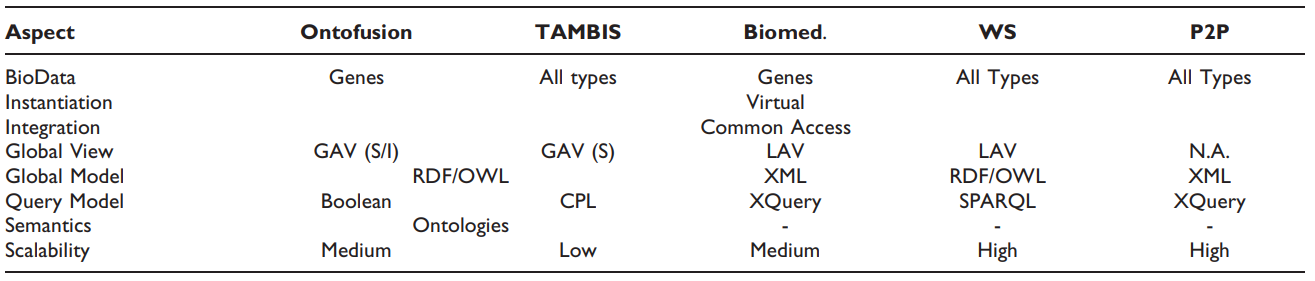
\includegraphics[scale=0.7]{img/Mediator based table}
                \caption{Σύγκριση των Mediator-based συστημάτων \cite{XMLbasedApproaches}}
            \end{figure}

        \subsubsection{Service-oriented συστήματα}
            Η Service-oriented αρχιτεκτονική προσφέρει μια τυποποιημένη μέθοδο για την ενσωμάτωση και των δεδομένων και του λογισμικού, θεωρώντας τα ως υπηρεσίες.
            Έτσι οι εφαρμογές θα τις συνδυάσουν για να υλοποιήσουν τις προβλεπόμενες εργασίες τους.

        \subsubsection{Peer-based συστήματα}
            Προσφέρουν μια αποκεντρωμένη προσέγγιση για την ενσωμάτωση δεδομένων μεταξύ διαφορετικών πηγών δεδομένων σε ένα δίκτυο.
            Η αποκέντρωση προσφέρει μεγαλύτερη ευελιξία και επεκτασιμότητα, ενώ δεν είναι απαραίτητη η δημιουργία μιας κεντρικής οντολογίας στην οποία πρέπει να μετατραπούν όλα τα δεδομένα.
            Από την άλλη, αυτά τα συστήματα δεν είναι τόσο αποδοτικά, καθώς η πολυπλοκότητα των δεδομένων είναι αυξημένη.


    \subsection{Παράμετροι για την ενοποίηση των δεδομένων}
        Κάποιες από τις παραμέτρους που επηρεάζουν την αρχιτεκτονική που θα χρησιμοποιήσουμε για την ενοποίηση των δεδομένων είναι \textbf{οι τύποι των δεδομένων} (όλα βασίζονται στο XML, αλλά διαφορετικά συστήματα ενοποίησης εστιάζουν σε διαφορετικούς τύπους δεδομένων όπως αλληλουχίες, γονιδιακές εκφράσεις κτλ),
            το \textbf{global model} (η μορφή της αναπαράστασης: relation-based (SQL), tree-based (XML), graph-based (RDF)), το \textbf{query model} (οι γλώσσες που χρησιμοποιούνται για την πρόσβαση στα δεδομένα όπως SQL, XQuery κτλ), η \textbf{επεκτασιμότητα} κ.α.

    \subsection{Εξειδικευμένα θέματα στην ενοποίηση XML δεδομένων}
        Το άρθρο κάνει αναφορά σε κάποια επιπλέον ζητήματα που αφορούν την ενοποίηση των δεδομένων που βασίζονται στο XML.

        Τίθονται θέματα που αφορούν την ασφάλεια των δεδομένων, την εξέλιξη των δεδομένων λόγω της δυναμικής φύσης τους, την αποτελεσματικότητα των ερωτήσεων (queries) που θέτουμε όπως επίσης και την έλλειψη -για την ώρα- μιας τυποποιημένης αρχιτεκτονικής που να εφαρμόζεται καθολικά.

    Σε κάθε περίπτωση, γίνεται σαφές πως το XML έχει ξεκάθαρα επιτύχει ως τη συντακτική κόλλα που συνδέει διάφορες πηγές με βιολογικά δεδομένα.
    Το αρνητικό είναι πως έχει δημιουργήσει μια μεγάλη ποικιλία διαφορετικών μορφών δεδομένων, κάτι που καθιστά δύσκολη την αποτελεσματική ενσωμάτωσή τους.
